\documentclass[12pt]{article}
\usepackage{graphicx}
\usepackage[left=3cm,top=3cm,right=3cm,bottom=3cm]{geometry}

\newcommand{\BEASTVersion}{2.0}
\newcommand{\TracerVersion}{1.5}
\newcommand{\FigTreeVersion}{1.3.1}

\begin{document}

\author{Alexei J Drummond and Remco Bouckaert}

\date{\today{}}

\title{Measurably evolving populations \label{chap.MEP}}
\maketitle



%%%%%%%%%%%%%%%%%%%%%%%%%%%%%%%%%%%%%%%%%%%%%
%%%
%%% EXERCISE - TIME-STAMPED DATA
%%%
%%%%%%%%%%%%%%%%%%%%%%%%%%%%%%%%%%%%%%%%%%%%%

\section{Time-stamped data}

This tutorial estimates the rate of evolution from a set of virus sequences which have been isolated at different points in time (heterochronous or time-stamped data). The data are 129 sequences from the G (attachment protein) gene of human respiratory
syncytial virus subgroup A (RSVA) from various parts of the world with isolation dates ranging from 1956-2002 \cite{Zlateva:2004uq,Zlateva:2005qy}.
RSVA causes infections of the lower respiratory tract causing symptoms that are often indistinguishable from the common cold. By age 3, nearly all children will be infected and a small percentage ($<3\%$) will develop more serious inflammation of the bronchioles requiring hospitalisation.

The aim of this tutorial is to obtain estimates for :

\begin{itemize}
\item the rate of molecular evolution
\item the date of the most recent common ancestor
\item the phylogenetic relationships with measures of statistical support.
\end{itemize}

The following software will be used in this tutorial:

\begin{itemize}
\item {\bf BEAST} - this package contains the BEAST program, BEAUti, DensiTree, TreeAnnotator and other utility programs. This tutorial is written for BEAST v{\BEASTVersion}, which has support for multiple partitions. It is available for download from \\* \texttt{http://beast2.cs.auckland.ac.nz/}.
\item {\bf Tracer} - this program is used to explore the output of BEAST (and other Bayesian MCMC programs). It graphically and
quantitively summarizes the distributions of continuous parameters and provides diagnostic information. At the time of
writing, the current version is v{\TracerVersion}. It is available for download from \texttt{http://beast.bio.ed.ac.uk/}.
\item {\bf FigTree} - this is an application for displaying and printing molecular phylogenies, in particular those obtained using
BEAST. At the time of writing, the current version is v{\FigTreeVersion}. It is available for download from \texttt{http://tree.bio.ed.ac.uk/}.
\end{itemize}

\subsection*{The NEXUS alignment}
The data is in a file called \texttt{RSV2.nex} and you can find it in the {\tt examples/nexus} directory in the directory where BEAST was installed. This file contains an alignment of 129 sequences from the G gene of RSVA virus, 629 nucleotides in length. Import this alignment into BEAUti. Because this is a protein-coding gene we are going to split the alignment into three partitions representing each of the three codon positions. To do this we will click the {\bf Split} button at the bottom of the {\bf Partitions} panel and then select the ``1 + 2 + 3 frame 3'' from the drop-down menu. This signifies that the first full codon starts at the third nucleotide in the alignment. This will create three rows in the partitions panel. You will have to re-link the tree and clock models across the three partitions (and name them ``tree'' and ``clock'' respectively) before continuing to the next step.

The partition panel should now look something like this:

\begin{center}
\includegraphics[scale=0.4,clip=true,trim=0 0 0 0]{figures/BEAUti_partition.png}%generated/
\end{center}

By default all the taxa are assumed to have a date of zero (i.e. the sequences are assumed to be sampled at the same time).
In this case, the RSVA sequences have been sampled at various dates going back to the 1950s. The actual year of sampling
is given in the name of each taxon and we could simply edit the value in the Date column of the table to reflect these.
However, if the taxa names contain the calibration information, then a convenient way to specify the dates of the sequences
in BEAUti is to click the checkbox {\bf Use tip dates} and then use the {\bf Guess} button at the top of the {\bf Tip Dates} panel. Clicking this will make a dialog box appear.

\medskip{}

\begin{center}
\includegraphics[width=0.6\textwidth]{figures/BEAUti_GuessDates.png}%generated/
\end{center}

\medskip{}

Select the option to {\it use everything}, choose ``after last'' from from drop-down box and type`s' into the corresponding text box. This will extract the trailing numbers from the taxon names after the last little 's', which are interpreted as the year (in this case since 1900) that the sample was isolated.

%For more information about the {\bf Guess Dates} facility see the Notes.
The dates panel should now look something like this:

\begin{center}
\includegraphics[scale=0.4,clip=true,trim=0 0 0 0]{figures/BEAUti_dates.png}%generated/
\end{center}


\subsection*{Setting the substitution model}
We will use the HKY model with empirical base frequencies for all three partitions. To do this first link the site partitions and then choose HKY and Empirical from the Subst Model and Frequencies drop-boxes. Also check the estimate box for the Mutation Rate and finally check the ``Fix mean mutation rate'' box. Then go back to Partitions panel and unlink the partitions.

\medskip{}

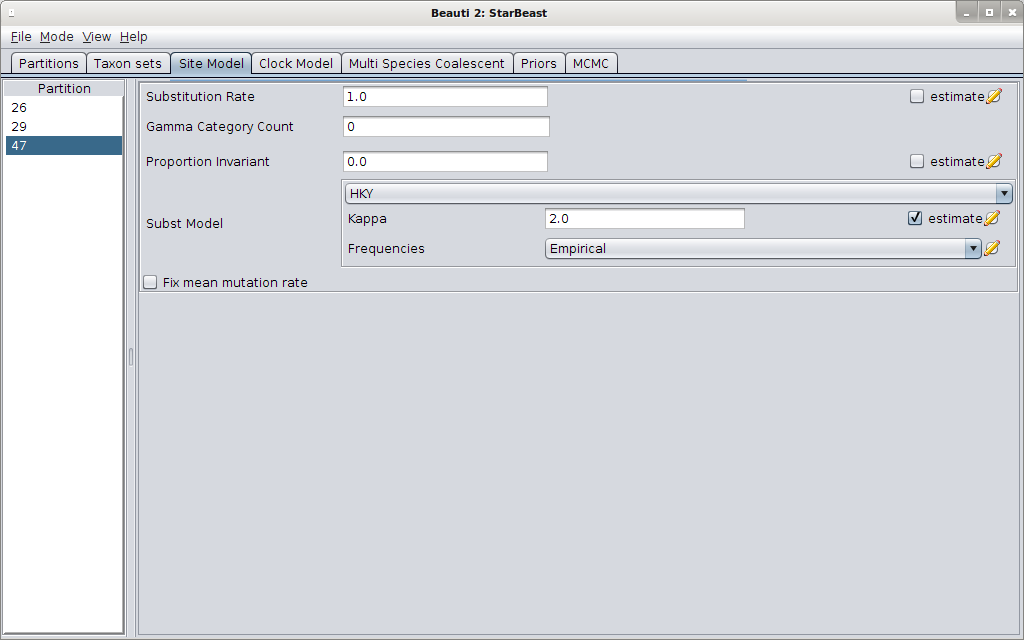
\includegraphics[width=\textwidth]{figures/BEAUti_Site_Model}%generated/

\medskip{}

\subsubsection{Priors }

To set up the priors, select the ``Priors'' tab.
Choose ``Coalescent Constant Population'' for the tree prior. Set the prior on the clockRate parameter to a log-normal with $M=-5$ and $S=1.25$. 

\medskip{}

\begin{center}
\includegraphics[width=0.8\textwidth]{figures/BEAUti_priors}%generated/
\end{center}

\medskip{}

\subsection{Setting the MCMC options}

For this dataset let's initially set the chain length to 2,000,000 as this will run 
reasonably quickly on most modern computers. Set the sampling frequencies for the screen to
to 1000, the trace log file to 400 and the trees file to 400.

\begin{center}
\includegraphics[width=0.8\textwidth]{figures/BEAUti_mcmc.png}%generated/
\end{center}


\subsection*{Running BEAST}

Save the BEAST file (e.g. \texttt{RSV2.xml}) and run it in BEAST.

\subsection*{Analysing the BEAST output}

Note that the effective sample sizes (ESSs) for many of the logged quantities are small (ESSs less than 100 will be highlighted in red by Tracer).
This is not good. A low ESS means that the trace contains a lot of correlated samples and thus may not represent the
posterior distribution well. In the bottom right of the window is a frequency plot of the samples which is expected given the
low ESSs is extremely rough.

If we select the tab on the right-hand-side labelled `Trace' we can view the raw trace, that is, the sampled values against the step in the MCMC chain.

\medskip{}

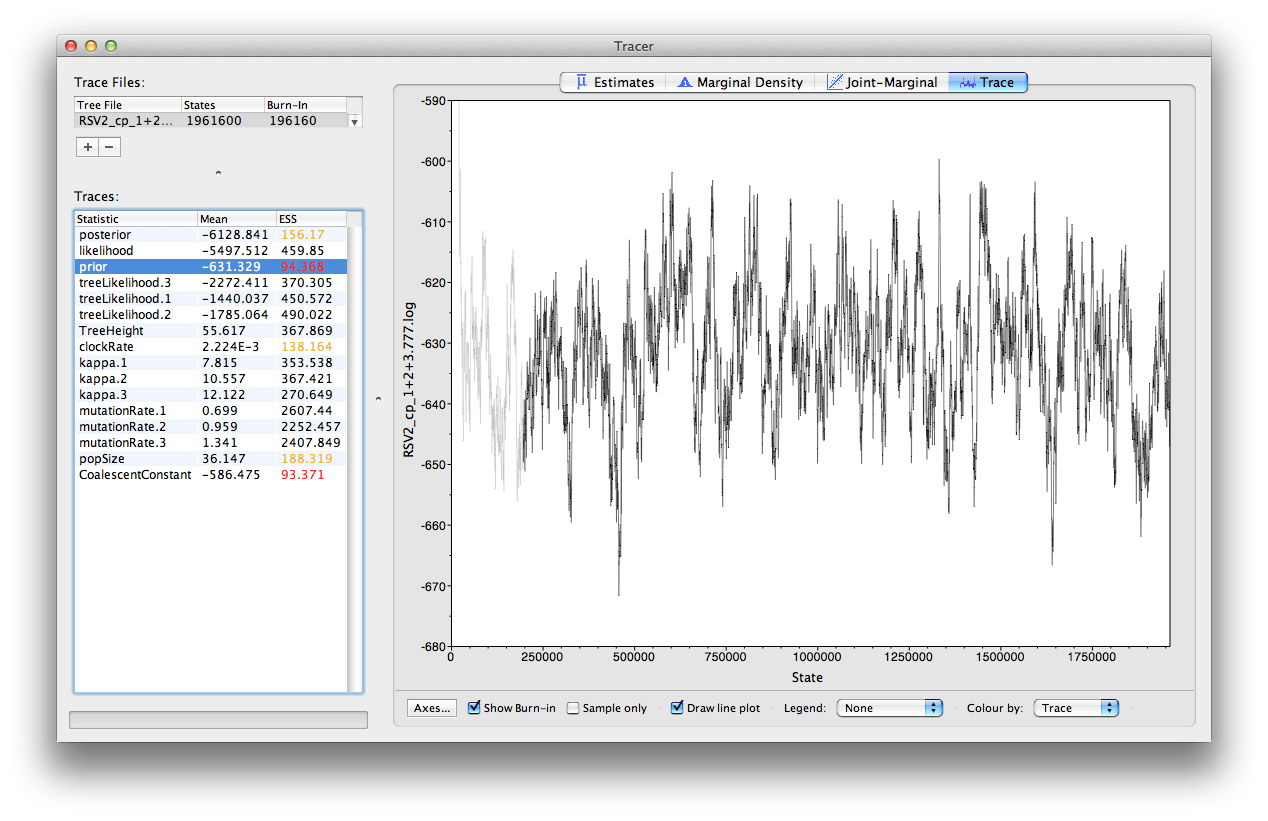
\includegraphics[width=\textwidth]{figures/Tracer1}

\medskip{}

Here you can see how the samples are correlated. There are 5000 samples in the trace (we ran the MCMC for 2,000,000
steps sampling every 400) but adjacent samples often tend to have similar values. The ESS for the absolute rate of evolution (clockRate) is about 138 so we are only getting 1 independent sample to every $36=5000/138$ actual samples). With a short run such as this one, it may also be the case that the default burn-in of 10\% of the chain length is inadequate. Not excluding enough of the start of the chain as burn-in will render estimates of ESS unreliable.

The simple response to this situation is that we need to run the chain for longer. Given the lowest ESS (for the constant coalescent prior) is 93, it
would suggest that we have to run the chain for at least twice the length to get reasonable ESSs that are $>$200. However it would be better to aim
higher so lets go for a chain length of 10,000,000. Go back to the {\bf MCMC} options section in BEAUti, and create a new BEAST
XML file with a longer chain length. Now run BEAST and load the new log file into Tracer (you can leave the old one loaded
for comparison). 

% Operator schedule for longer run
%Operator                                                              Tuning	#accept	#reject	#total	acceptance rate
%ScaleOperator_treeScaler.t:tree                                       0.749 	2979	357860	360839	0.008 Try setting scaleFactor to about 0.866
%ScaleOperator_treeRootScaler.t:tree                                   0.665 	32937	326676	359613	0.092 Try setting scaleFactor to about 0.816
%Uniform_UniformOperator.t:tree                                              	1933260	1667698	3600958	0.537 
%SubtreeSlide_SubtreeSlide.t:tree                                      3.689 	305813	1493386	1799199	0.17 
%Exchange_narrow.t:tree                                                      	443444	1358454	1801898	0.246 
%Exchange_wide.t:tree                                                        	778	360870	361648	0.002 
%WilsonBalding_WilsonBalding.t:tree                                          	1829	357480	359309	0.005 
%ScaleOperator_StrictClockRateScaler.c:clock                           0.774 	81499	278426	359925	0.226 
%UpDownOperator_strictClockUpDownOperator.c:clock                      0.805 	4122	355324	359446	0.011 Try setting scaleFactor to about 0.897
%ScaleOperator_KappaScaler.s:RSV2_1                                    0.382 	2848	9239	12087	0.236 
%DeltaExchangeOperator_FixMeanMutationRatesOperator                    0.314 	52671	187054	239725	0.22 
%ScaleOperator_KappaScaler.s:RSV2_2                                    0.434 	3178	8799	11977	0.265 
%ScaleOperator_KappaScaler.s:RSV2_3                                    0.447 	2911	9176	12087	0.241 
%ScaleOperator_PopSizeScaler.t:tree                                    0.570 	85369	275921	361290	0.236 
%Total calculation time: 1822.878 seconds

Click on the Trace tab and look at the raw trace plot.

\medskip{}

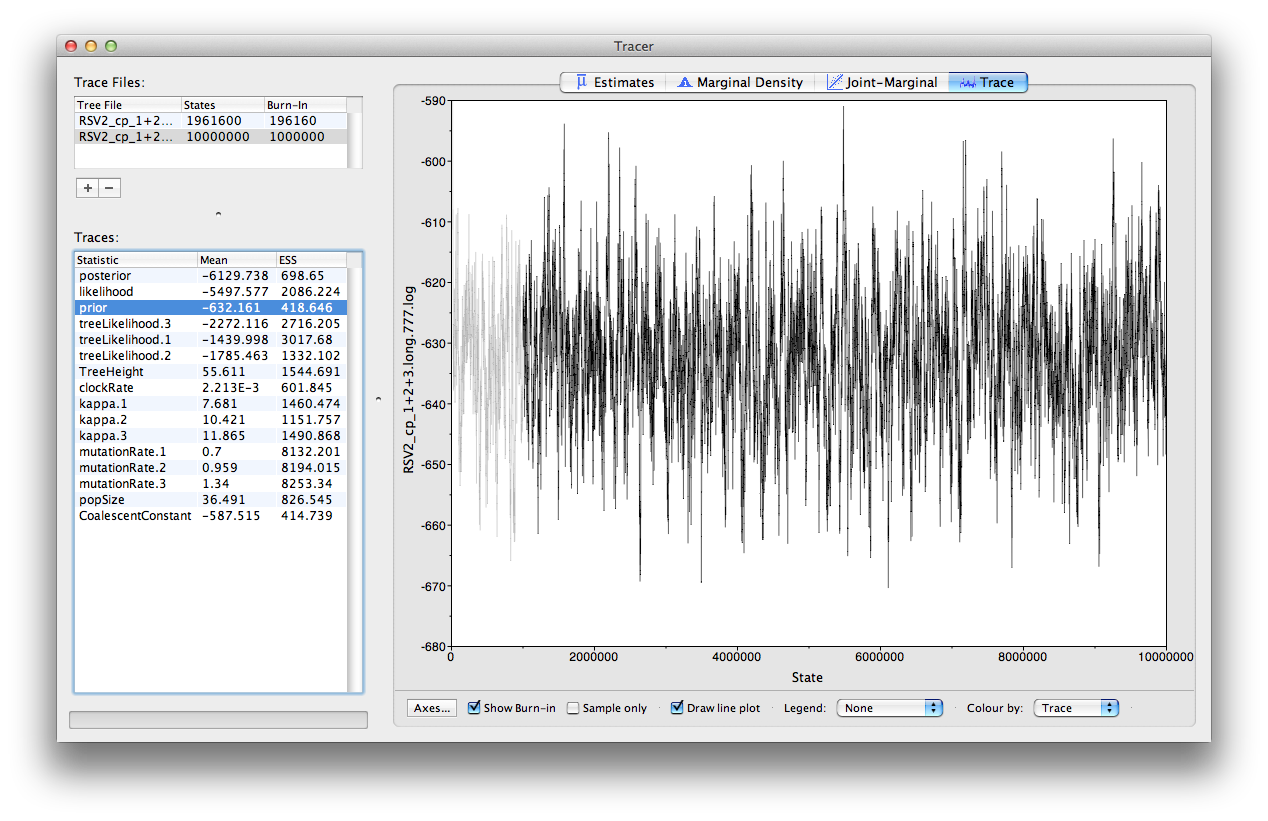
\includegraphics[width=\textwidth]{figures/Tracer2}

\medskip{}

Again we have chosen options that produce 5000 samples and with an ESS of about 419 there is still auto-correlation
between the samples but $>$400 effectively independent samples will now provide a very good estimate of the posterior distribution.
There are no obvious trends in the plot which would suggest that the MCMC has not yet converged, and there are no significant long range 
fluctuations in the trace which would suggest poor mixing.

As we are satisfied with the mixing we can now move on to one of the parameters of interest:
substitution rate. Select \texttt{clockRate} in the left-hand table. This is the average substitution rate across all sites in the
alignment. Now choose the density plot by selecting the tab labeled {\it Marginal Density}. This shows a plot of the marginal posterior probability
density of this parameter. You should see a plot similar to this:

\medskip{}

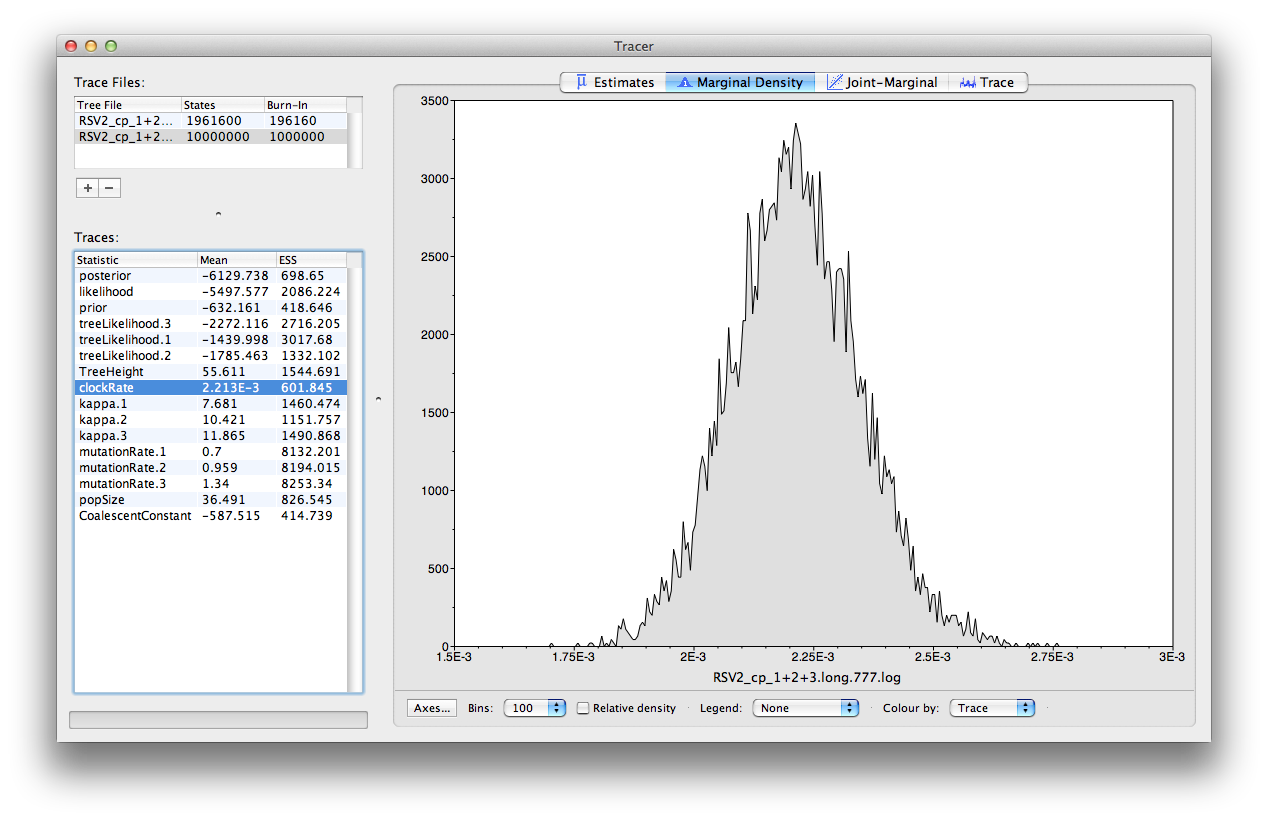
\includegraphics[width=\textwidth]{figures/Tracer_density}

\medskip{}

As you can see the posterior probability density is roughly bell-shaped. There is some sampling noise which would be
reduced if we ran the chain for longer or sampled more often but we already have a good estimate of the mean and HPD interval. You can overlay
the density plots of multiple traces in order to compare them (it is up to the user to determine whether they are comparable on the the same axis or not). Select the relative substitution rates for all three codon positions in the table to the left (labelled
\texttt{mutationRate.1}, \texttt{mutationRate.2} and \texttt{mutationRate.3}). You will now see the posterior probability densities for the relative
substitution rate at all three codon positions overlaid:

\medskip{}

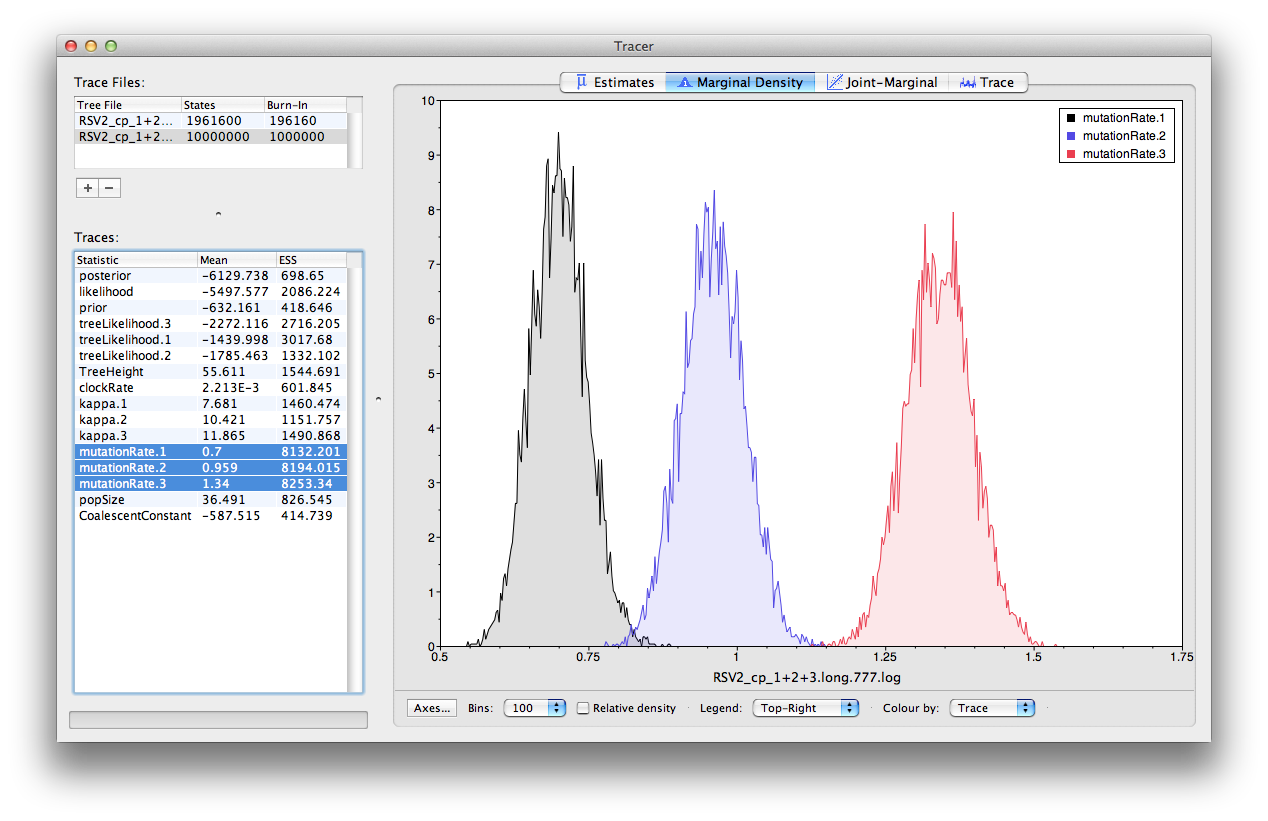
\includegraphics[width=\textwidth]{figures/Tracer_relativeRates}

\subsection*{Summarizing the trees}

Use the program TreeAnnotator to summarize the tree and view the results in Figtree (Figure \ref{fig:RSV2tree}).

\begin{figure}

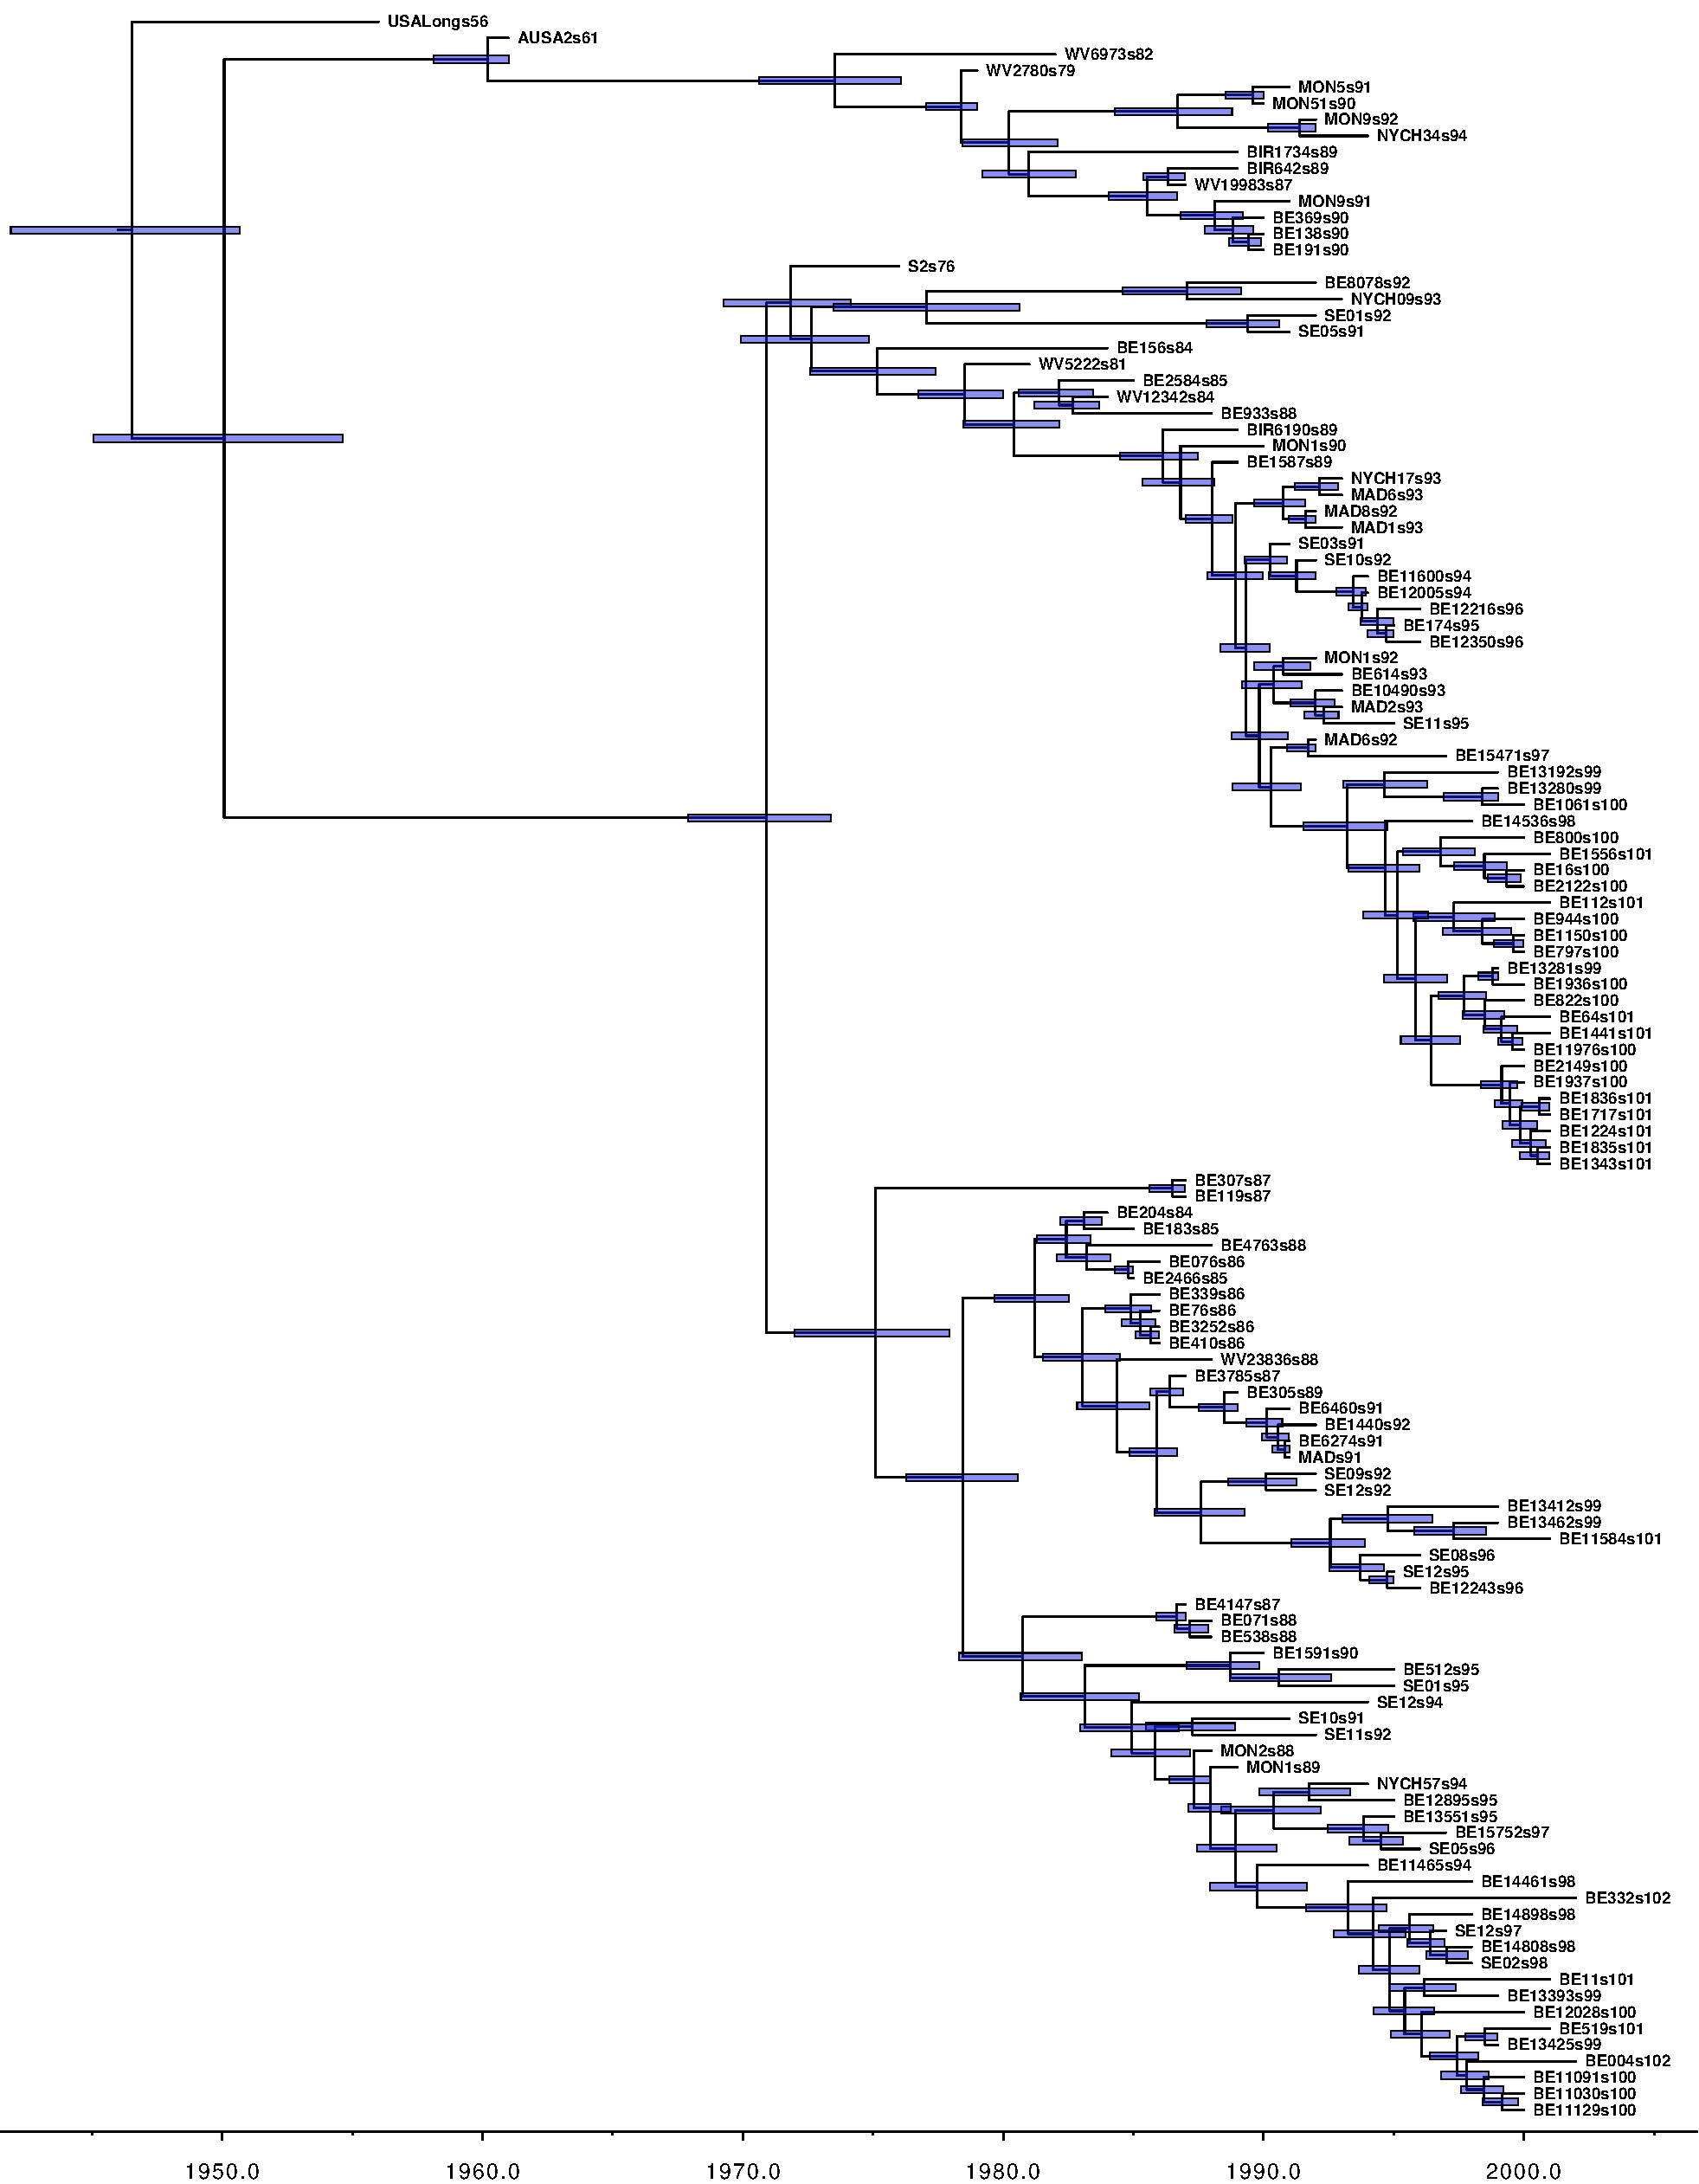
\includegraphics[width=\textwidth]{figures/RSV2_mcc_tree.pdf}

\caption{The Maximum clade credibility tree for the G gene of 129 RSVA-2 viral samples. }
\label{fig:RSV2tree}
\end{figure}


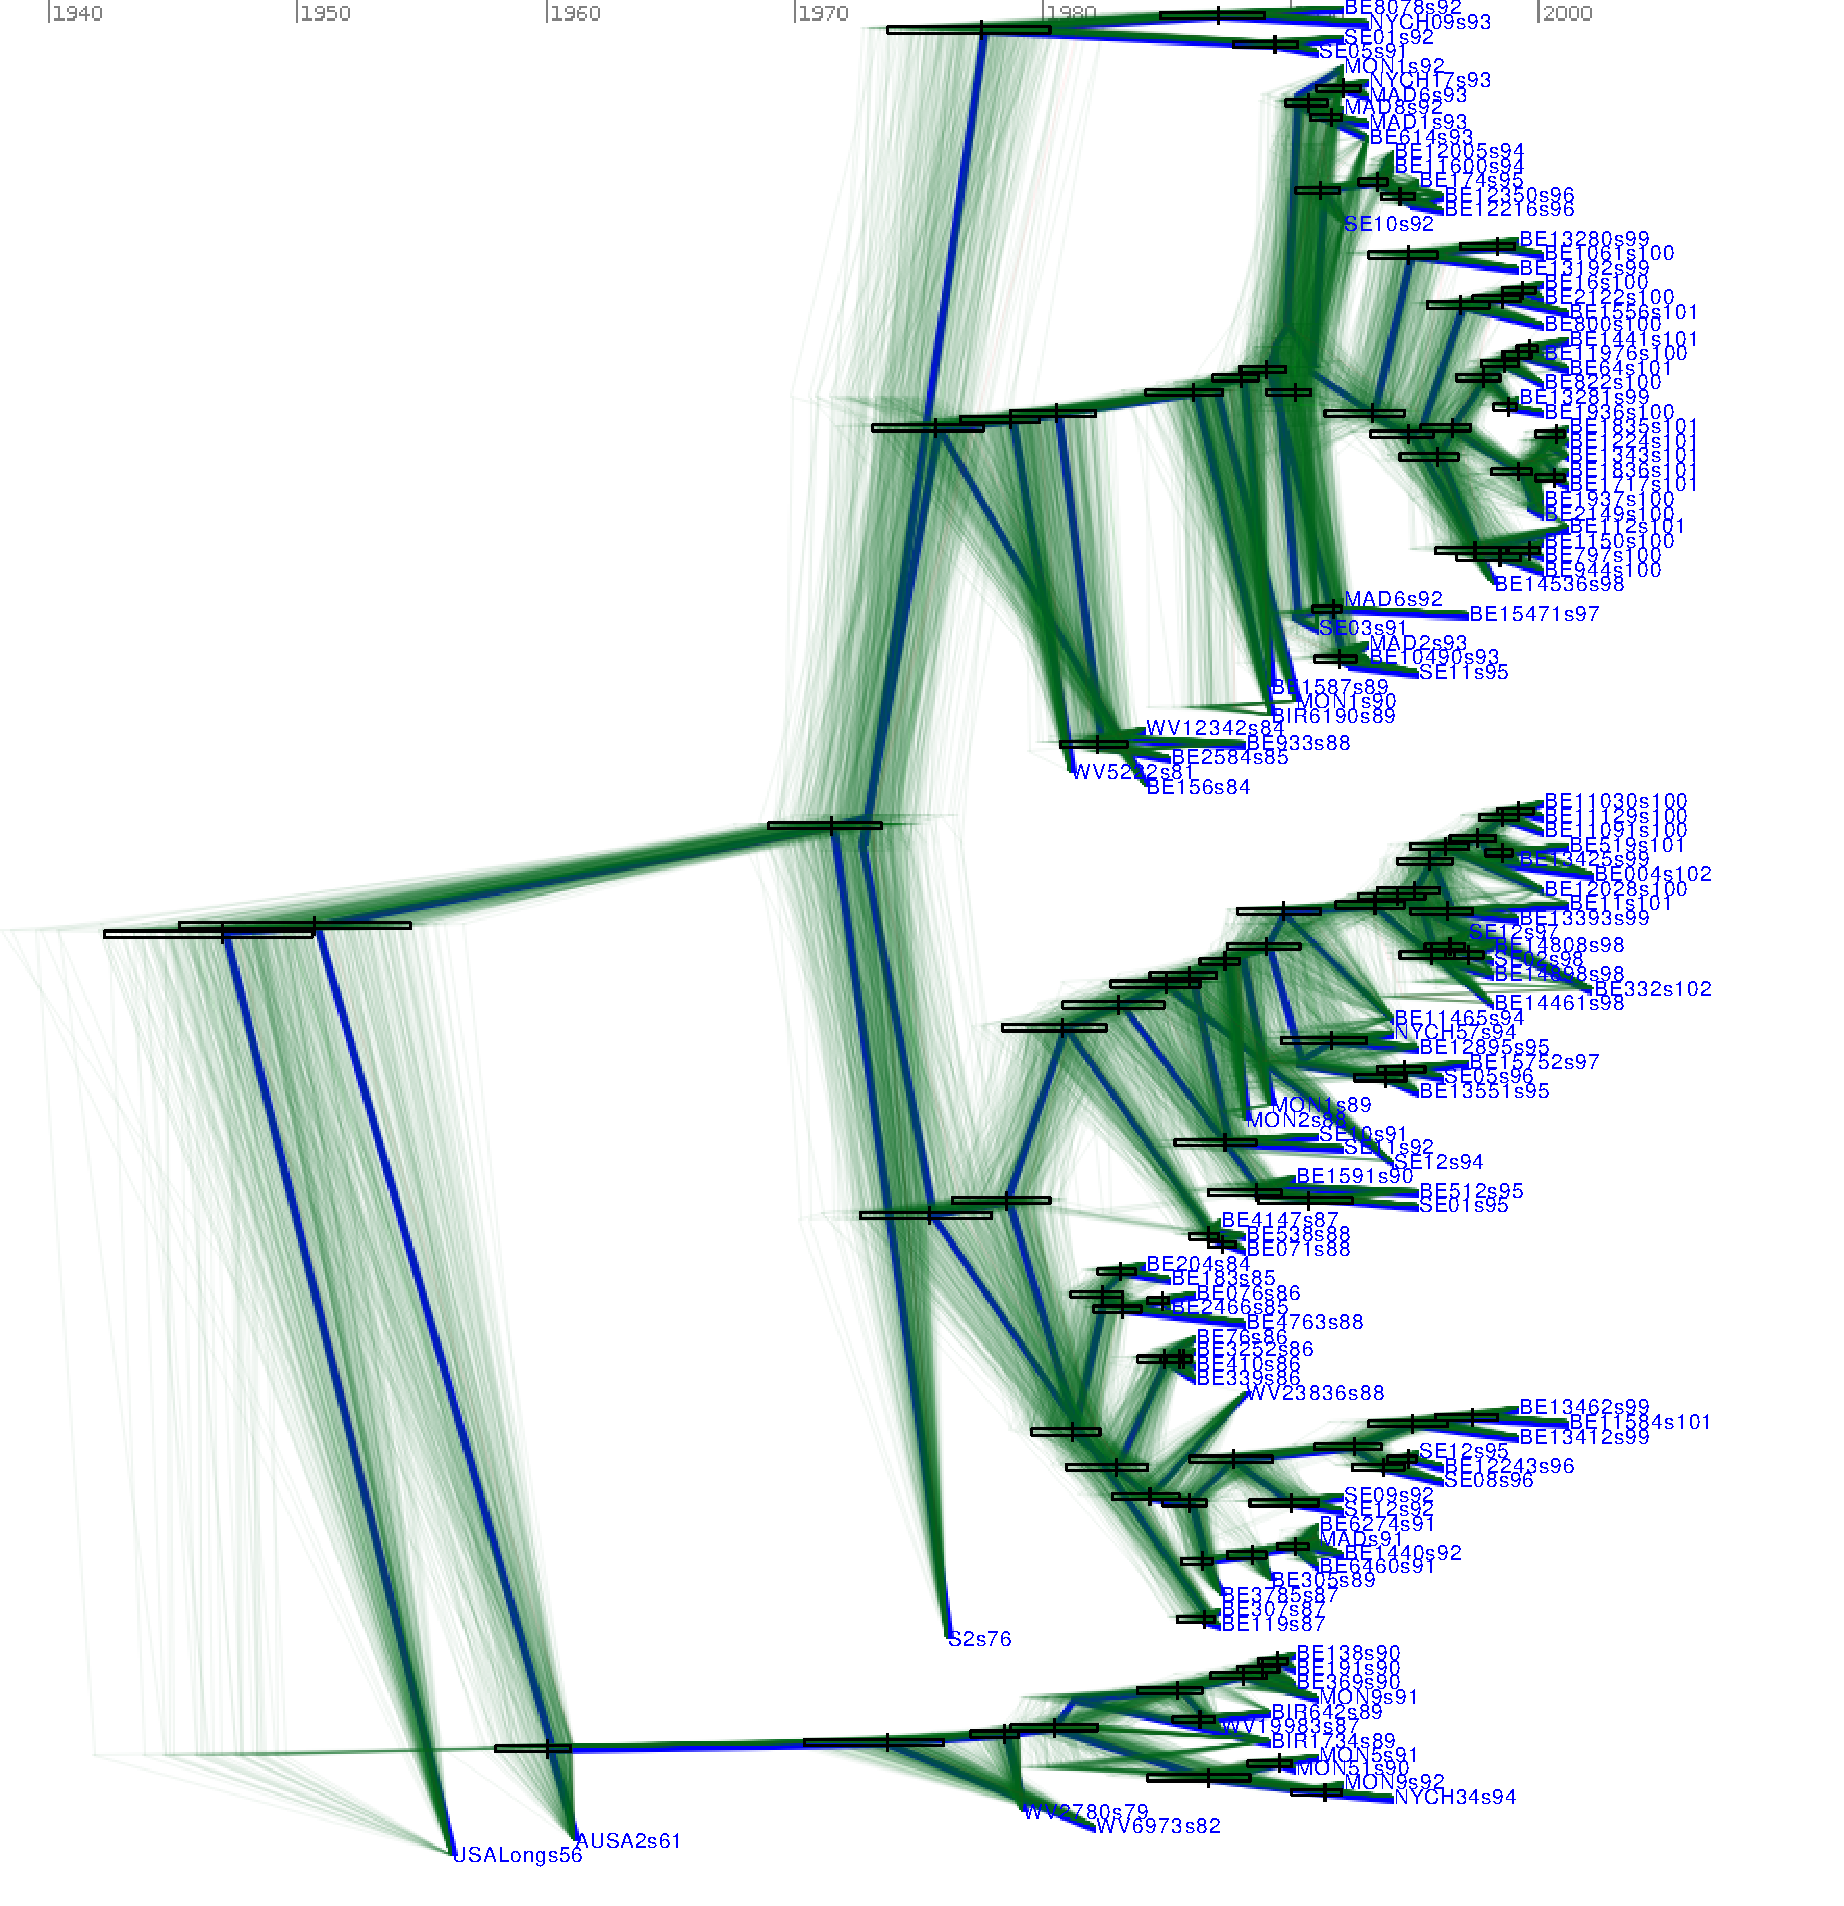
\includegraphics[width=\textwidth]{figures/DensiTree.pdf}
DensiTree with clade height bars for clades with over 50\% support.
Root canal tree represents maximum clade credibility tree.


\subsection*{Questions}

\textit{In what year did the common ancestor of all RSVA viruses sampled live? What is the
95\% HPD?}

\framebox(420,60){}


\subsection*{Bonus section: Bayesian Skyline plot}

We can reconstruct the population history using the Bayesian Skyline plot. In order to do so,
load the XML file into BEAUti, select the priors-tab and change the tree prior from 
coalescent with constant population size to coalescent with Bayesian skyline.
Note that an extra item is added to the priors called `Markov chained population sizes'
which is a prior that ensures dependence between population sizes.

\begin{center}
\includegraphics[scale=0.5,clip=true,trim=0 0 0 0]{figures/BEAUti_priors2.png}%generated/
\end{center}

By default the number of groups used in the skyline analysis is set to 5, To change this,
select menu View/Show Initialization panel and a list of parameters is shown. Select
{\tt bPopSizes.t:tree} and change the dimension to 3. Likewise, selection {\tt bGroupSizes.t:tree}
and change its dimension to 3. The dimensions of the two parameters should be the same.
More groups mean more population changes can be detected, but it also means more parameters
need to be estimated and the chain runs longer. The extended Bayesian skyline plot
automatically detects the number of changes, so it could be used as an alternative
tree prior.

\begin{center}
\includegraphics[scale=0.5,clip=true,trim=0 0 0 0]{figures/BEAUti_init.png}%generated/
\end{center}


This analysis requires a bit longer to converge, so change the MCMC chain length to 10 million,
and the log intervals for the trace-log and tree-log to 10 thousand. 
Then, save the file and run BEAST.


To plot the population history, load the log file in tracer and select the menu 
Analysis/Bayesian Skyline Reconstruction.

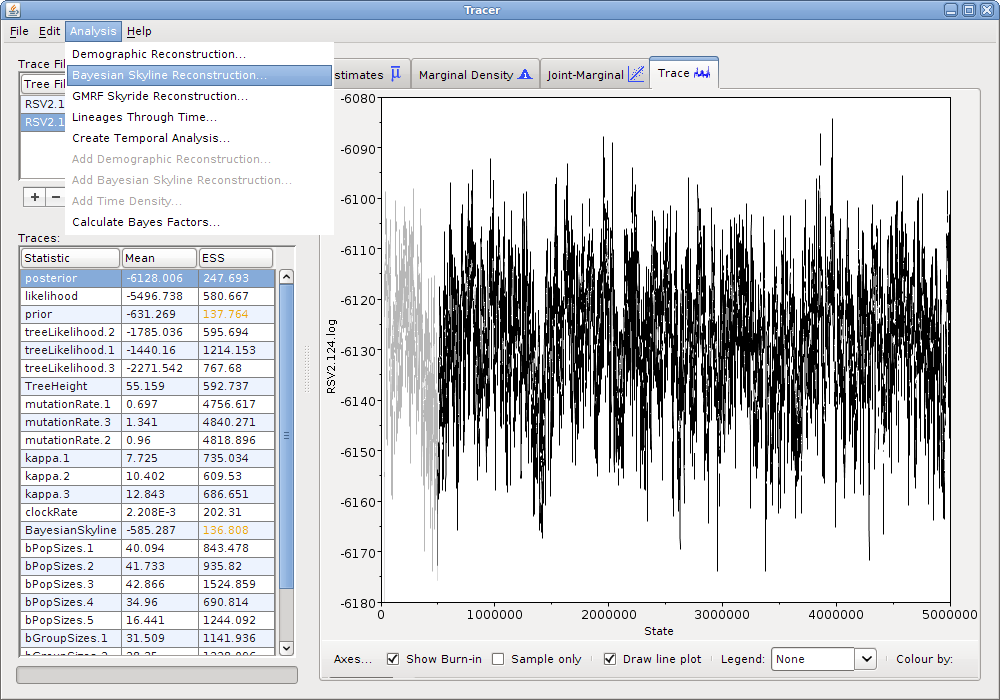
\includegraphics[scale=0.5,clip=true,trim=0 300 0 0]{figures/tracerBSP1.png}

A dialog is shown where you can specify the tree file associated with the log file.
Also, since the youngest sample is from 2002, change the entry for age of youngest
tip to 2002.

\begin{center}
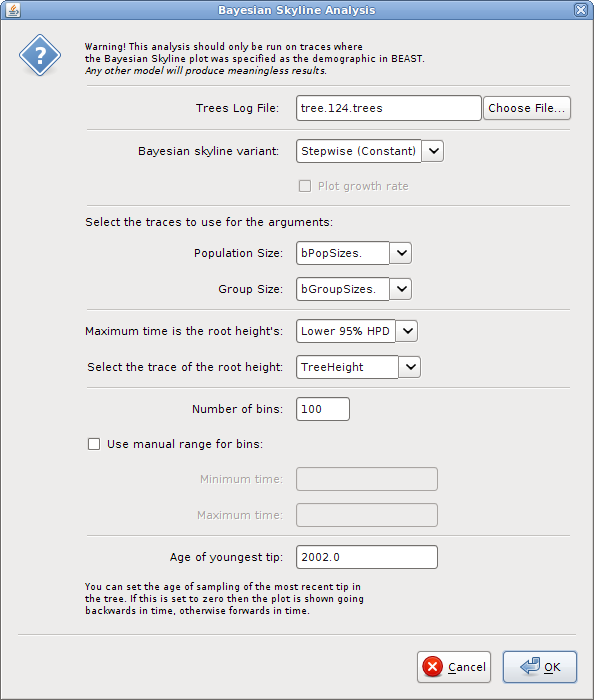
\includegraphics[width=0.6\textwidth]{figures/tracerBSP2.png}
\end{center}

After some calculation, a graph appears showing population history where the median
and 95\% HPD intervals are plotted. After selecting the `solid interval' checkbox, the
graph should look something like this.

\begin{center}
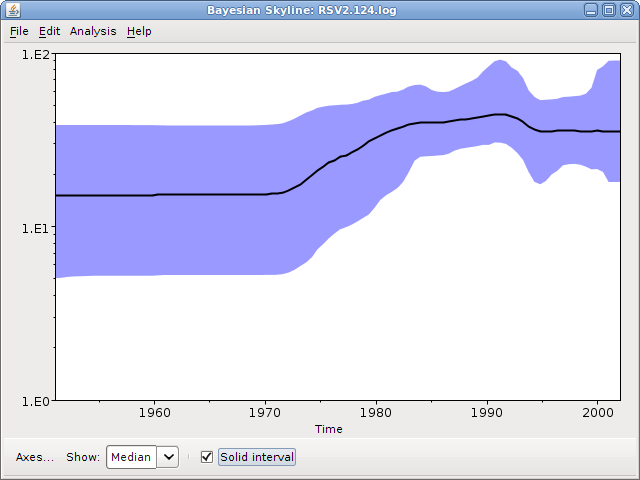
\includegraphics[width=0.7\textwidth]{figures/tracerBSP3.png}
\end{center}


\subsection*{Questions}
\vspace{5 mm}

\textit{By what amount did the effective population size of RSVA grow from 1970 to 2002 according to the BSP?}
 
\vspace{5 mm}
\framebox(420,30){}
\vspace{5 mm}

\textit{What are the underlying assumptions of the BSP? Are the violated by this data set?}
 
\vspace{5 mm}
\framebox(420,90){}
\vspace{5 mm}



\subsection{Exercise}
Change the Bayesian skyline prior to extended Bayesian skyline plot (EBSP) prior and run
till convergence. EBSP produces an extra log file, called EBSP.\$(seed).log where \$(seed)
is replaced by the seed you used to run BEAST.
A plot can be created by running the EBSPAnalyser utility, and loading the output file
in a spreadsheet.

How many groups are indicated by the EBSP analysis?
This is much lower than for BSP. How does this affect the population history plots?

\bibliographystyle{amsplain} 
\bibliography{MEPs}

\end{document}

